\newcommand{\content}
{
    % добавляем нумерацию
    \AddToShipoutPicture{
        \begin{textblock*}{1cm}(19.5cm,28.6cm) % Ширина блока, координаты (x, y)
                \centering 
                \number\numexpr\thepage+1\relax
        \end{textblock*}
    }

    % добавляем шифр
    \AddToShipoutPicture{
        \begin{textblock*}{10cm}(9cm,28.2cm) % Ширина блока, координаты (x, y)
            \centering
            \chipher
        \end{textblock*}
    }

    % шифр на 1ый лист
    \begin{textblock*}{10cm}(9cm,28.2cm) % Ширина блока, координаты (x, y)
        \centering
        \chipher
    \end{textblock*}

    \newpage
    \section{\MakeUppercase{Введение}}
    {
        Современная индустрия общественного питания активно интегрирует цифровые технологии для улучшения качества обслуживания клиентов и оптимизации внутренних бизнес-процессов. Создание интеллектуальных систем, таких как веб-приложения для кафе, является актуальным направлением, учитывая возрастающий спрос на автоматизацию и удобные сервисы. Клиенты предпочитают комфортные способы заказа и взаимодействия с заведениями, а администраторы и персонал нуждаются в эффективных инструментах управления.
        
        Разработка приложения, функционирующего через платформу Telegram, позволит решить множество задач: от упрощения процесса оформления заказов для клиентов до автоматизации работы сотрудников и администраторов. Это особенно важно в условиях высокой конкуренции на рынке, где скорость и удобство обслуживания играют ключевую роль. Кроме того, использование Telegram как платформы обеспечит широкую доступность и минимальные затраты на обучение пользователей.
        
        Целью работы является создание интеллектуальной системы, которая интегрирует возможности управления кафе в единый интерфейс, предоставляя персонализированные функции для клиентов, работников и администраторов. Реализация такого подхода позволит значительно повысить эффективность работы заведения, сократить ошибки и ускорить процесс обслуживания.  
        
        Таким образом, разработка данного приложения актуальна как для улучшения клиентского опыта, так и для оптимизации работы предприятия в сфере общественного питания.
    }

    \newpage
    \section{\MakeUppercase{Постановка задачи}}

    Целью проекта является разработка интеллектуальной системы веб-приложения для кафе на базе платформы Telegram, с использованием технологии Flutter для клиентской части и Firebase для хранения данных и серверной логики. Данная система обеспечит эффективное взаимодействие между клиентами, сотрудниками и администрацией заведения.

    Для достижения поставленной цели необходимо решить следующие задачи:  
    \begin{itemize}
        \item \textbf{исследование и анализ технологий:}
        \begin{itemize}
            \item изучить особенности платформы Telegram для создания Mini App, включая работу с Bot API и взаимодействие через интерактивные кнопки;
            \item исследовать возможности Flutter как инструмента для создания адаптивных интерфейсов, подходящих для Telegram Mini App;
            \item рассмотреть функциональность Firebase, включая использование Fire-store для хранения данных, Firebase Functions для серверной логики и Firebase Authentication для безопасной аутентификации.
        \end{itemize}

        \item \textbf{проектирование архитектуры приложения:}
        \begin{itemize}
            \item разработать структуру базы данных на Firestore, включающую таблицы для пользователей, меню, заказов и сотрудников;
            \item спроектировать серверную логику на Firebase Functions для обработки заказов, управления статусами и отправки уведомлений;
            \item определить схему взаимодействия между Telegram Mini App, Firebase и Flutter.
        \end{itemize}

        \item \textbf{разработка интерфейса:}
        \begin{itemize}
            \item используя Flutter, создать интуитивно понятный интерфейс для взаимодействия с Telegram Mini App;
            \item реализовать разделение интерфейса по ролям пользователей: клиенты, сотрудники, администраторы;
            \item обеспечить доступность интерфейса для работы на разных устройствах.
        \end{itemize}

        \item \textbf{разработка функционала:}
        \begin{itemize}
            \item реализовать систему заказа блюд через Telegram Mini App;
            \item создать интерфейсы для управления заказами сотрудниками кафе;
            \item разработать административные инструменты для редактирования меню, управления сотрудниками и настройки кафе.
        \end{itemize}

        \item \textbf{интеграция с базой данных:}
        \begin{itemize}
            \item настроить безопасное взаимодействие между клиентской частью и Firestore;
            \item реализовать обработку и синхронизацию данных через Firebase Func-tions;
            \item проверить надёжность хранения данных и соответствие структуры базы требованиям приложения.
        \end{itemize}

        \item \textbf{тестирование системы:}
        \begin{itemize}
            \item выполнить тестирование Telegram Mini App для проверки корректности работы интерактивных кнопок и взаимодействия с пользователями;
            \item проверить функционал, разработанный на Flutter, включая стабильность интерфейса и его адаптивность;
            \item провести тестирование работы Firebase, включая производительность базы данных, функции аутентификации и обработку событий через серверные функции.
        \end{itemize}

        \item \textbf{оптимизация и доработка:}
        \begin{itemize}
            \item устранить выявленные в ходе тестирования недостатки;
            \item оптимизировать запросы к базе данных Firebase для повышения скорости обработки данных;
            \item улучшить пользовательский опыт, основываясь на обратной связи от тестирования.
        \end{itemize}
    \end{itemize}


    \newpage
    \section{\MakeUppercase{Выбор и описание используемых инструментов}}
    {
        \subsection{Telegram}
        {
            Telegram выбран как основная платформа для взаимодействия с пользователями из-за его уникальных преимуществ решения существующих проблем в предметной области. В отличие от традиционных подходов, требующих установки отдельных приложений для каждого кафе, Telegram уже широко распространён и установлен на устройствах пользователей. Это избавляет клиентов от необходимости скачивать дополнительное программное обеспечение, занимать место на устройстве и проходить трудоёмкую регистрацию. Автоматическая авторизация через существующий аккаунт Telegram упрощает вход в систему, делая процесс максимально удобным и быстрым. Платформа создаёт интуитивно понятный способ взаимодействия для всех пользователей - от клиентов до администраторов кафе, существенно облегчая пользовательский опыт и снижая затраты на поддержку системы.
        }

        \subsection{Flutter}
        {
            Flutter выбран как инструмент разработки с принципиально важной стратегической перспективой расширения проекта. Этот фреймворк от Google не только позволяет создавать высокопроизводительные и адаптивные интерфейсы для Telegram-приложения, но и обеспечивает возможность быстрого масштабирования проекта. Использование Flutter дает преимущество практически моментального развертывания web-версии приложения, а в дальнейшем - создания мобильных приложений для iOS и Android без существенных переработок кода. Это означает, что начальное решение для Telegram может быть легко трансформировано в полноценную экосистему приложений для кафе с единой логикой и дизайном.
        }

        \subsection{Firebase}
        {
            Firebase был выбран как решение, которое обеспечивает надёжность, масштабируемость и централизованное управление информацией для системы взаимодействия кафе. Платформа предоставляет комплексный инструментарий для хранения данных, который гарантирует:
            \begin{itemize}
                \item моментальную синхронизацию информации между всеми пользователями;
                \item высокий уровень безопасности данных;
                \item возможность горизонтального масштабирования без значительных технических затрат;
                \item простоту интеграции с различными платформами и сервисами.
            \end{itemize}

            Использование Firebase решает проблемы централизованного управления меню, заказами, правами доступа сотрудников и администраторов, создавая единое информационное пространство для всех участников системы.
        }
    }


    \newpage
    \section{\MakeUppercase{Разработка приложения}}
    В данном разделе описан процесс разработки веб-приложения для автоматизации работы кафе, включая как серверную, так и клиентскую части.

    \subsection{Разработка структуры базы данных}
    {
        Для хранения данных пользователей, заказов, меню и сотрудников было выбрано использование облачной базы данных Firebase. Она позволяет эффективно управлять данными в реальном времени, обеспечивая масштабируемость и безопасность.
        
        Схема базы данных, изображенная на рисунке 4.1, включает несколько ключевых сущностей: 
        \begin{itemize}
            \item \textbf{пользователи Users:} хранение информации о клиентах, включая их имя, email, номер телефона и роль клиент или администратор;
            \item \textbf{заказы Orders:} хранение информации о заказах, связанных с пользователями, и содержащих пункты из меню;
            \item \textbf{меню MenuItems:} хранение информации о пунктах меню название, цена, категория;
            \item \textbf{сотрудники Employees:} хранении информации о сотрудниках кафе, включая их роль и контактные данные.
        \end{itemize}

        Связи между сущностями в базе данных:
        \begin{itemize}
            \item пользователь может сделать несколько заказов, поэтому связь 1 ко многим между Users и Orders;
            \item каждый заказ может включать несколько пунктов меню, поэтому связь многие ко многим между Orders и MenuItems;
            \item сотрудники могут обрабатывать заказы, поэтому связь многие ко многим между Employees и Orders.
        \end{itemize} 

        
        \begin{figure}[H]
            \centering
            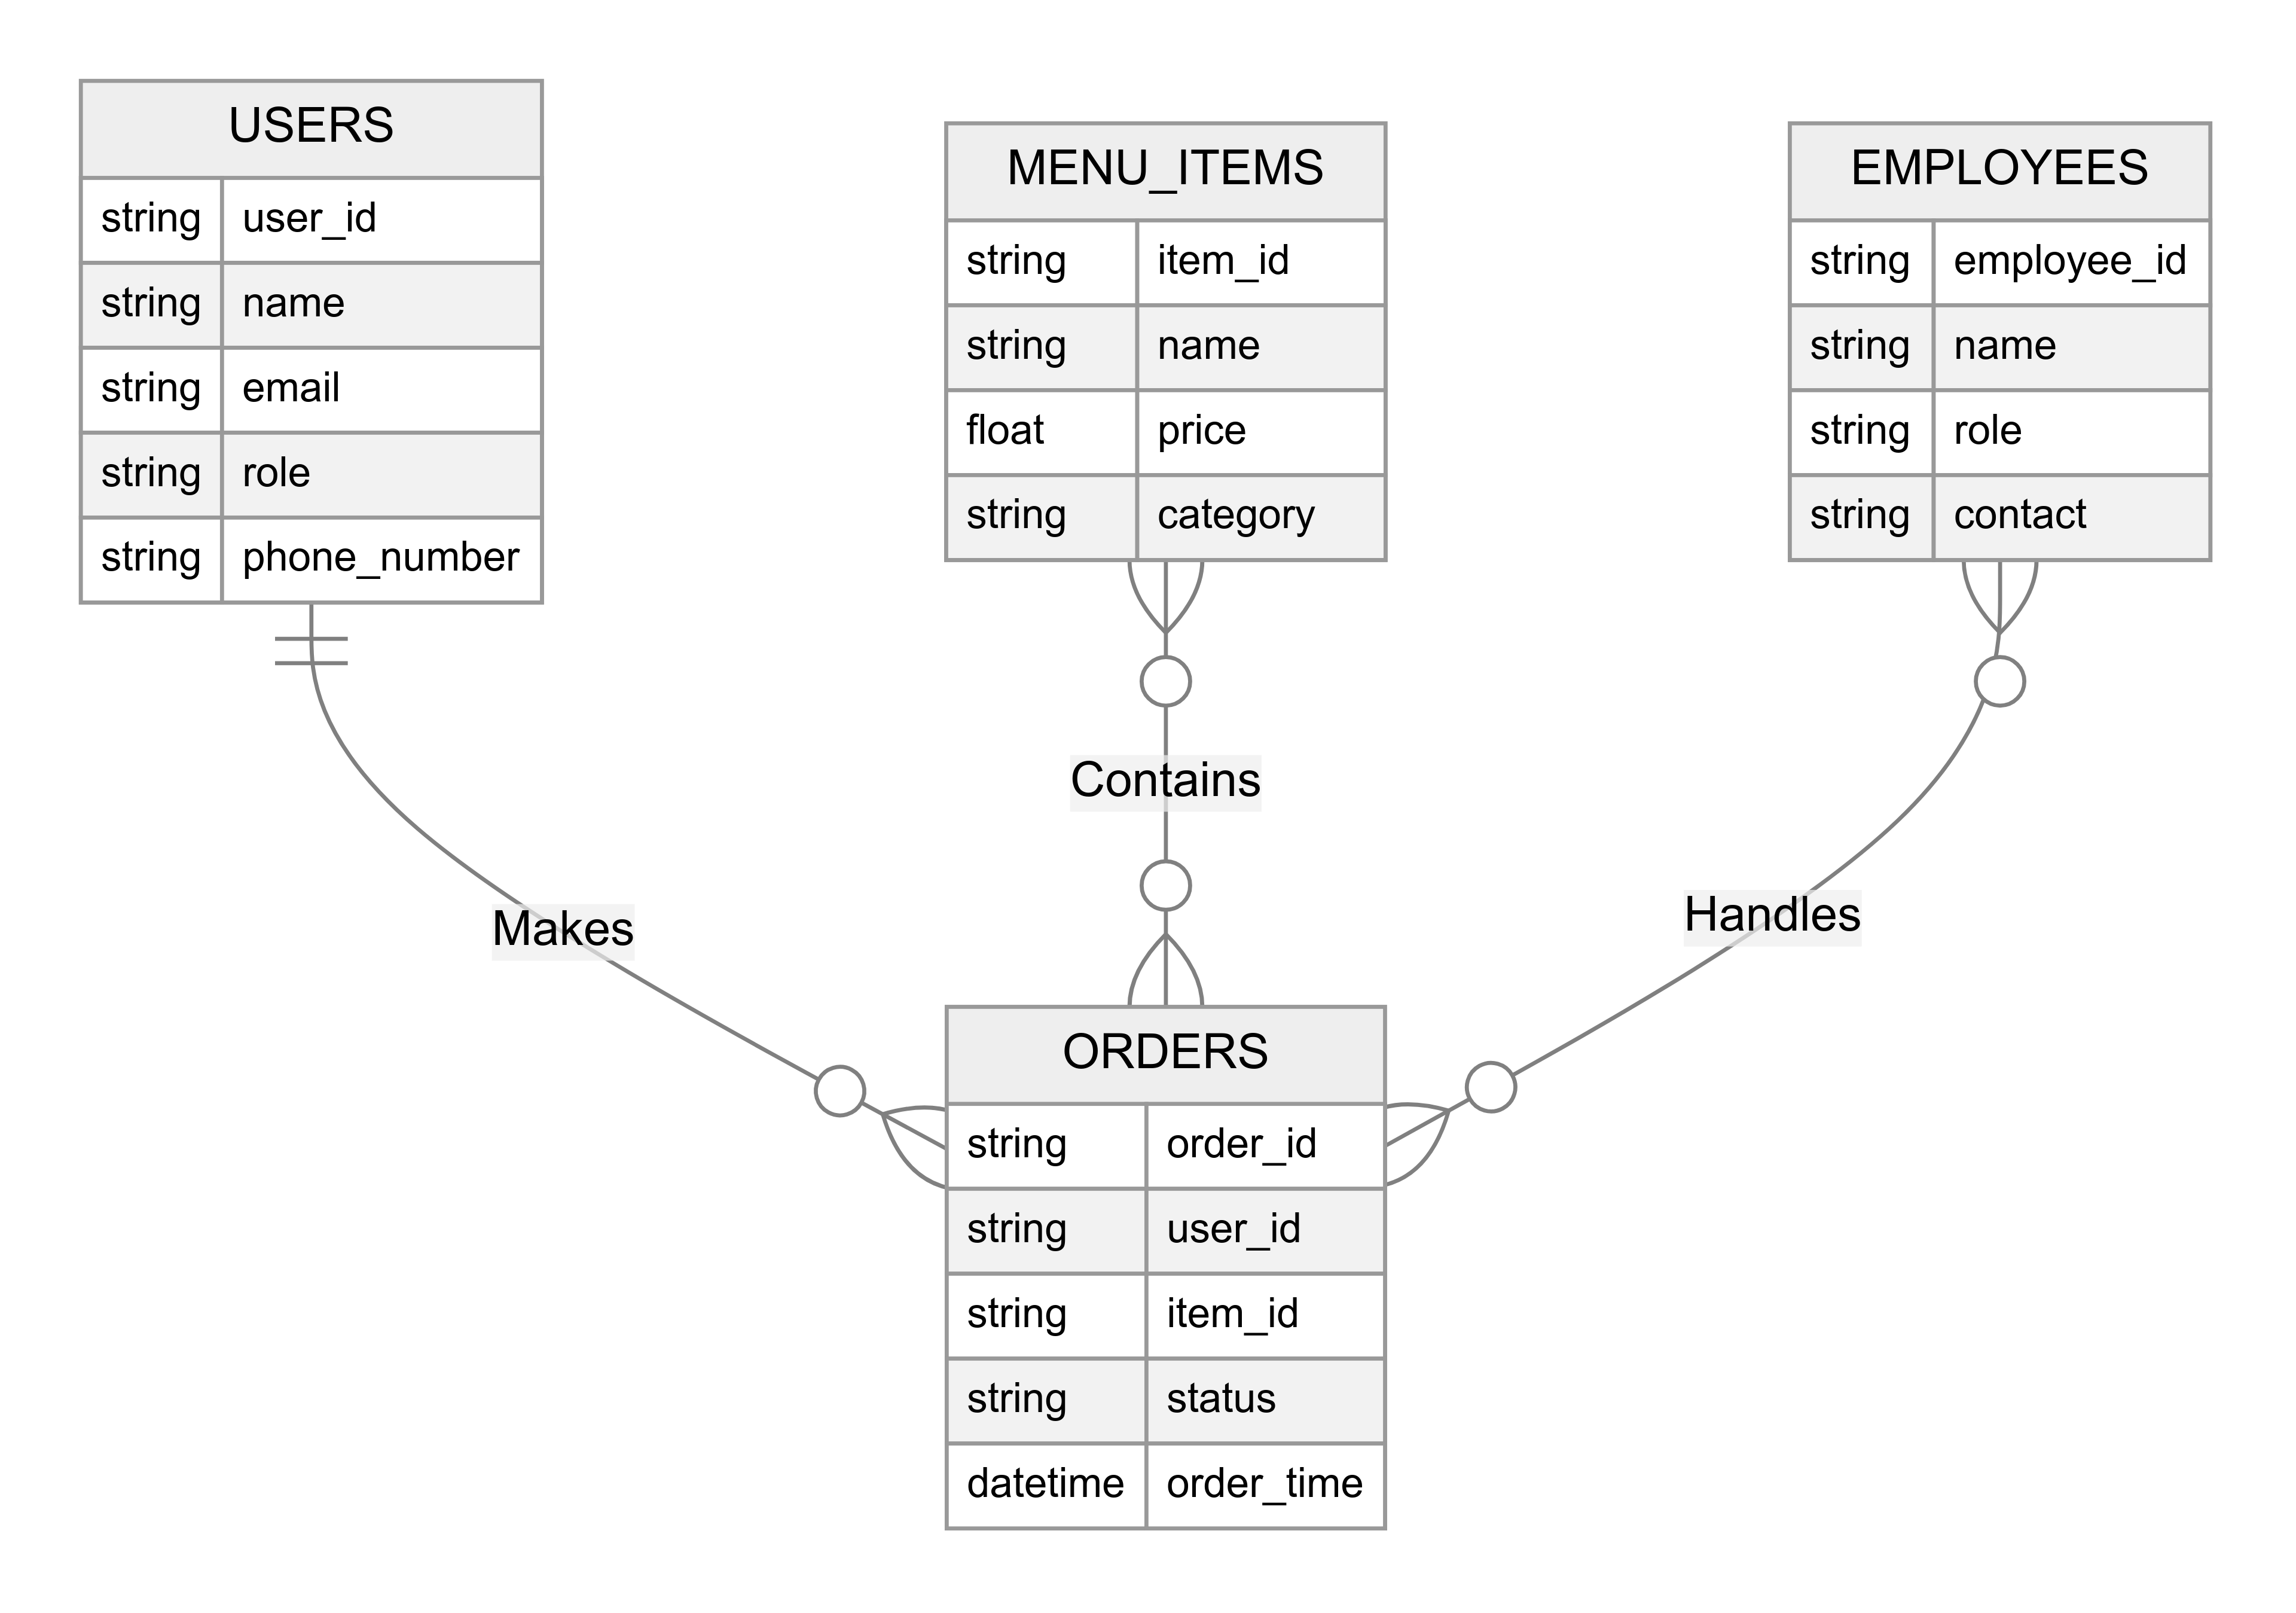
\includegraphics[width=1\textwidth]{assets/database.png} 
            \caption{Структура базы данных}
        \end{figure}
    }

    \subsection{Разработка логики работы системы} 
    {
        Логика работы системы приложения, изображенная на рисунке 4.2, описывает ключевые этапы взаимодействия пользователей с приложением, включая процесс оформления заказа, его обработки сотрудниками и уведомления пользователей. Краткое описание этапов:
        \begin{itemize}
            \item пользователь выбирает блюда из меню;
            \item эти блюда добавляются в корзину;
            \item затем пользователь оформляет заказ.
            \item Если пользователь не авторизован, система запрашивает его данные для входа.
            \item После авторизации заказ отправляется на сервер.
            \item Система проверяет статус заказа, и если он обработан, уведомляет пользователя.
            \item В случае, если заказ в процессе, сотрудник кафе его обрабатывает.
            \item После завершения обработки заказа сотрудник подтверждает выполнение, и пользователь получает уведомление.
        \end{itemize}

        \begin{figure}[H]
            \centering
            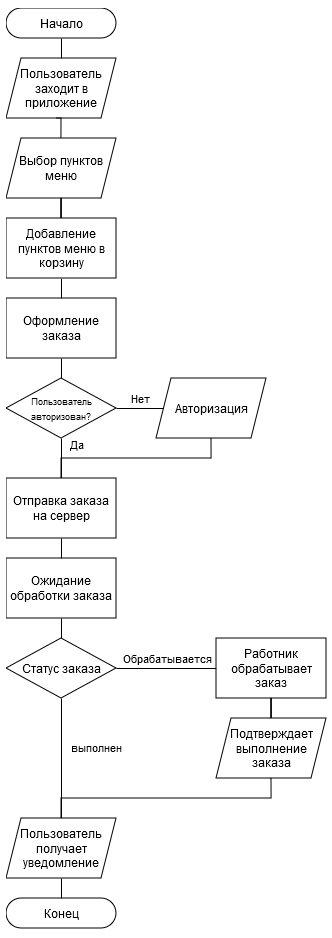
\includegraphics[height=1.2\textwidth]{assets/scheme.png} 
            \caption{Схема работы системы}
        \end{figure}
    }

    \subsection{Разработка клиентской части приложения}
    {
        Для разработки клиентской части приложения был выбран фреймворк Flutter, который позволяет быстро создавать кроссплатформенные приложения с одним кодом для различных платформ. Основные этапы разработки клиентской части:
        \begin{itemize}
            \item \textbf{интерфейс пользовател:} был разработан простой и интуитивно понятный интерфейс для выбора блюд (рисунок 4.3), оформления заказов (рисунок 4.4) и управления пользователями. Интерфейс был разработан с помощью Flutter и пакета Flutter Telegram Web для взаимодействия с Telegram;
            \item \textbf{взаимодействие с сервером:} для обмена данными с сервером использовались пакеты firebase\_core и cloud\_firestore, которые позволяют отправлять запросы и получать ответы от базы данных Firebase;
            \item \textbf{аутентификация:} для безопасности данных и авторизации пользователей применена система Firebase Authentication, которая предоставляет удобные средства для регистрации и входа в приложение; 
        \end{itemize}
        \begin{figure}[H]
            \centering
            \begin{minipage}{0.45\textwidth}
                \centering
                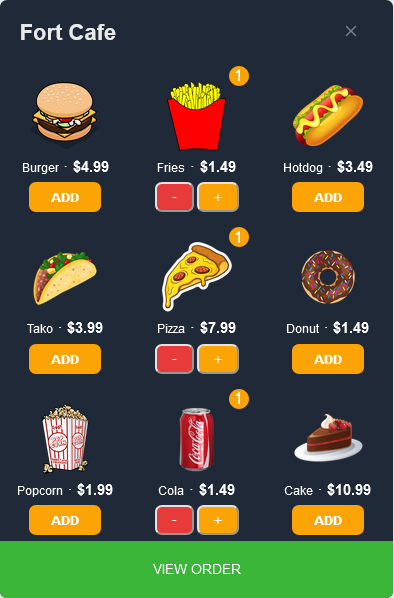
\includegraphics[width=\textwidth]{assets/menu.png}
                \caption{Экран меню}
                \label{fig:login_page}
            \end{minipage}
            \hfill
            \begin{minipage}{0.45\textwidth}
                \centering
                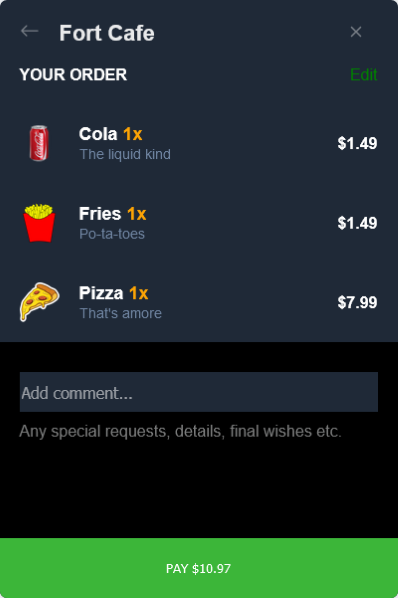
\includegraphics[width=\textwidth]{assets/order.png}
                \caption{Экран заказа}
                \label{fig:enter_data}
            \end{minipage}
        \end{figure}
    }

    \newpage
    \section{\MakeUppercase{Тестирование приложения}}

    В этом разделе рассматривается процесс тестирования веб-приложения, включая как функциональное, так и интеграционное тестирование. В ходе тестирования проверялись различные аспекты работы системы, такие как корректность выполнения операций, взаимодействие с базой данных, а также производительность и безопасность приложения. Тестирование включало следующие этапы:
    \begin{itemize}
        \item \textbf{функциональное тестирование:} при функциональном тестировании были обнаружены незначительные недостатки в работе интерфейса и логики приложения. В частности, возникали проблемы с корректным отображением обновлений корзины на разных устройствах и некорректной обработкой авторизации при оформлении заказа. Были исправлены выявленные недостатки и улучшен механизм обновления состояния корзины и логика обработки авторизации, что существенно повысило удобство использования приложения;
        \item \textbf{интеграционное тестирование:} интеграционное тестирование выявило проблемы взаимодействия приложения с базой данных Firebase. Основные сложности были связаны с некорректным сохранением заказов и задержками в обновлении статусов. Для решения этих проблем была оптимизирована логика обработки транзакций и усовершенствован механизм отслеживания изменений статусов заказа, что обеспечило более надежную и быструю работу системы;
        \item \textbf{тестирование производительности:} в ходе тестирования производительности обнаружены задержки при работе с большими объемами данных и высокой нагрузке. Были проведены оптимизация запросов к базе данных, внедрение кэширование и улучшение алгоритмов обработки заказов. Эти изменения значительно ускорили работу приложения и повысили его отзывчивость при одновременной работе множества пользователей;
        \item \textbf{безопасность:} тестирование безопасности показало необходимость усиления защиты от потенциальных веб-атак. Были внедрены дополнительные механизмы фильтрации и проверки входных данных, что существенно повысило защищенность персональной информации пользователей.
    \end{itemize}

    Проведенное тестирование позволило выявить и устранить ряд недостатков, существенно улучшив качество, производительность и безопасность приложения. Система готова к эксплуатации и обеспечивает надежную работу всех ключевых функций.\newpage
        
    \section{\MakeUppercase{Заключение}}
    {
        В ходе выполнения курсовой работы была достигнута основная цель - создание интеллектуальной системы управления кафе через веб-приложение в Telegram. Проведенное исследование полностью подтвердило актуальность разработки цифровых решений для оптимизации процессов в сфере общественного питания.

        Разработанное приложение представляет собой комплексное решение, которое объединяет функционал для клиентов, сотрудников и администраторов, существенно упрощая процессы взаимодействия внутри кафе и повышая качество сервиса. Использование платформы Telegram обеспечило широкую доступность приложения, минимальные затраты на обучение пользователей и интуитивно понятный интерфейс.

        Техническая реализация проекта базируется на современных технологиях разработки, таких как Flutter и Firebase, что гарантирует высокую производительность, масштабируемость и надежную защиту данных пользователей. Клиенты получили удобный инструмент для быстрого оформления заказов, сотрудники - эффективный механизм управления заказами, а администраторы - полный контроль над работой заведения.

        Проведенное тестирование подтвердило эффективность разработанного решения. Система полностью готова к внедрению и может быть успешно применена в различных заведениях общественного питания.

        Таким образом, цель курсовой работы была полностью достигнута, а разработанное приложение демонстрирует высокий потенциал для оптимизации работы кафе и улучшения качества обслуживания клиентов. Результаты исследования подтверждают актуальность и перспективность цифровизации сферы общественного питания через интеллектуальные веб-приложения.
    }

    \newpage
    \section{Список использованной литературы}
    \sloppy
    {
        \begin{enumerate}
            \item Telegram Bot API Documentation [Электронный ресурс]. – Режим доступа: \url{https://core.telegram.org/bots/api}. – Дата доступа: 19.11.2024.
            \item Flutter Documentation [Электронный ресурс]. – Режим доступа: \url{https://docs.flutter.dev/}. – Дата доступа: 19.11.2024.
            \item Firebase Documentation [Электронный ресурс]. – Режим доступа: \url{https://firebase.google.com/docs}. – Дата доступа: 19.11.2024.
            \item Dart Programming Language Guide [Электронный ресурс]. – Режим доступа: \url{https://dart.dev/guides}. – Дата доступа: 19.11.2024.
        \end{enumerate}
    }
}